\section{Integration}

\subsection{Construction and Properties}

  \subsubsection{Simple Functions}

    Remember that Riemann integration is characterized by the approximation of step functions, which are the "building blocks" of Riemann integrable functions. To define the Lebesgue integral, we will consider a generalization of step functions called \textit{simple functions}. A function will be Lebesgue integrable if it can be approximated by these simple functions in some appropriate way. 

    \begin{definition}[Simple Functions]
      For $A \subset X$ (any subset, not just in some $\sigma$-algebra), the \textbf{characteristic}, or \textbf{indicator} \textbf{function} of $A$ is the function $1_A : X \longrightarrow \mathbb{R}$ defined 
      \begin{equation}
        1_A (x) = \begin{cases} 1 & \text{ if } x \in A \\ 0 & \text{ if else} \end{cases}
      \end{equation}
      A function $\phi: \mathbb{R} \longrightarrow \mathbb{R}$ is called a \textbf{simple function} if it is a finite linear combination of characteristic functions. 
      \begin{equation}
        \phi = \sum_{i=1}^n a_i 1_{A_i}
      \end{equation}
    \end{definition}

    \begin{lemma}[Measurability on Simple Functions]
      Now, let $(X, \mathcal{A})$ be a measurable space. Then, 
      \begin{equation}
        \phi = \sum_{i=1}^n a_i 1_{A_i} : (X, \mathcal{A}) \longrightarrow \mathbb{R}
      \end{equation}
      is measurable if all $A_i$ are measurable, i.e. $A_i \in \mathcal{A}$ for all $i$. 
    \end{lemma}
    \begin{proof}
      Let $T$ be an open set in $\mathbb{R}$. Then, for characteristic function $1_A$, 
      \begin{equation}
        1_A^{-1} (T) = \begin{cases} 
        \emptyset & \text{ if } 0, 1 \not\in T \\
        A & \text{ if } 1 \in T, 0 \not\in T \\
        X \setminus A & \text{ if } 0 \in T, 1 \not\in T \\
        X & \text{ if } 0, 1 \in T
        \end{cases}
      \end{equation}
      and so $1_A$ must be measurable if $A \in \mathcal{A}$ (which also by definition implies that $A^c = X \setminus A \in \mathcal{A}$). If $1_{A_i}$ is measurable, then the linear combination of measurable functions is also measurable. 
    \end{proof}

    Also observe that the coefficients need not be unique, since we can write 
    \begin{equation}
      1 \cdot 1_{[0, 1]} + 1 \cdot 1_{[0.5, 1]} = 1 \cdot 1_{[0, 0.5]} + 2 \cdot 1_{[0.5, 1]}
    \end{equation}
    If the $E_i$'s are disjoint, then this decomposition is unique and is called the \textbf{standard representation} of $\phi$. 

    \begin{example}[Step Function as Simple Function]
      For $a, b \in \mathbb{R}$, with $a < b$, let $f: [a, b] \longrightarrow \mathbb{R}$ be a step function. That is, there exists a partition $a = x_0 < x_1 < \ldots < x_n = b$ and constants $c_1, c_2, \ldots, c_n \in \mathbb{R}$ s.t. $f(x) = c_i$ for all $x \in (x_{i-1}, x_i)$ and each $i = 1, \ldots, n$. Then, $f$ is equal to the following simple function, taken over all open intervals and the points $x_j$ at the boundary of each interval. 
      \begin{equation}
        f = \sum_{i=1}^n c_i 1_{(x_{i-1}, x_i)} + \sum_{j=0}^n f(x_j) 1_{\{x_j\}}
      \end{equation}
      If we ignore the behavior of $f$ on the partition points $x_j$'s, then $f$ agrees almost everywhere with the simple function 
      \begin{equation}
        \sum_{i=1}^n c_i 1_{(x_{i-1}, x_i)}
      \end{equation}
    \end{example}

    If the $A_i$'s above are just intervals in $\mathbb{R}$, then $\phi$ reduces to a step function. But the entire problem with intervals is that they are too coarse. We can't work with them, so we generalize them to all measurable sets in $(X, \mathcal{A})$. The Riemann integral is built on an approximation scheme of a function, which we usually want to be continuous to satisfy this approximation, and so, if we want to build an approximation scheme for Lebesgue integrals, we want a similar scheme, i.e. if we take a sequence of simple measurable functions, I can get arbitrarily close to any measurable function $f$. This is exactly what we show below. 

    \begin{theorem}
      If $f: (X, \mathcal{A}) \longrightarrow [0, \infty]$ is measurable, there are simple measurable functions $f_k : (X, \mathcal{A}) \longrightarrow [0, \infty)$ s.t. 
      \begin{equation}
        f_k \leq f_{k+1} \text{ and } f = \lim_{k \rightarrow \infty} f_k
      \end{equation}
      where the inequalities and limits are pointwise. 
    \end{theorem}
    \begin{proof}
      We give a general picture of this proof for a function $f: \mathbb{R} \longrightarrow [0, \infty]$. We can first divide the codomain of the graph below into segments of $t = 1, 2, \ldots$, and take the preimage of all these units under $f$ to get $f_1$. More specifically, $A_1^t = f^{-1} ([t, \infty])$ for all $t$. By measurability of $f$, $A_1^t$ is measurable, and we can assign $f_1 = 1_{A^1_1} + 1_{A_1^2} \leq f$. 
      \begin{center}
        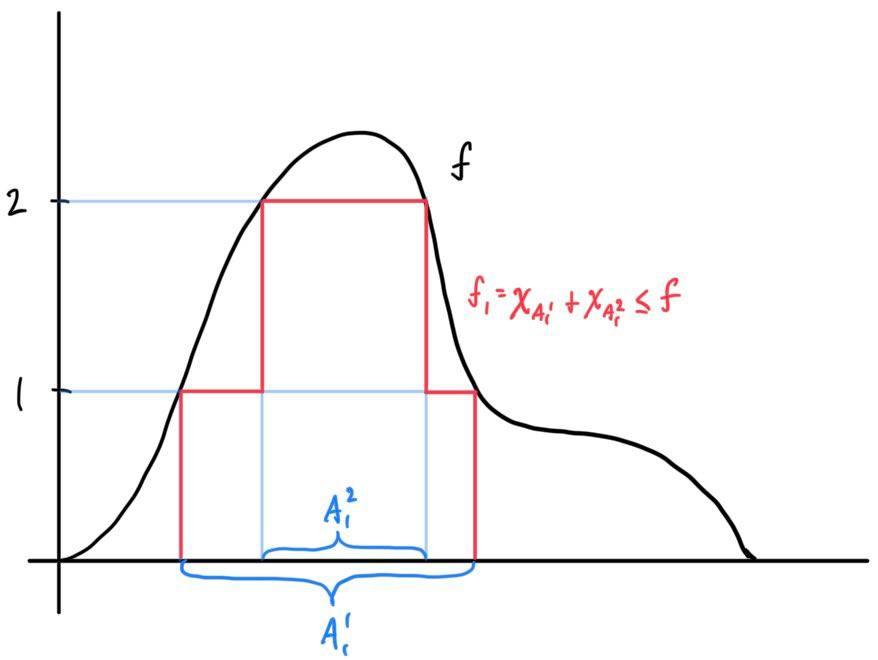
\includegraphics[scale=0.23]{img/Lebesgue_1.jpg}
      \end{center}
      Doing this again with finer subintervals of the codomain gives us, with $f_2 = 1_{A_2^1} + 1_{A_2^2} + 1_{A_2^3} + 1_{A_2^4} \leq f$. 
      \begin{center}
        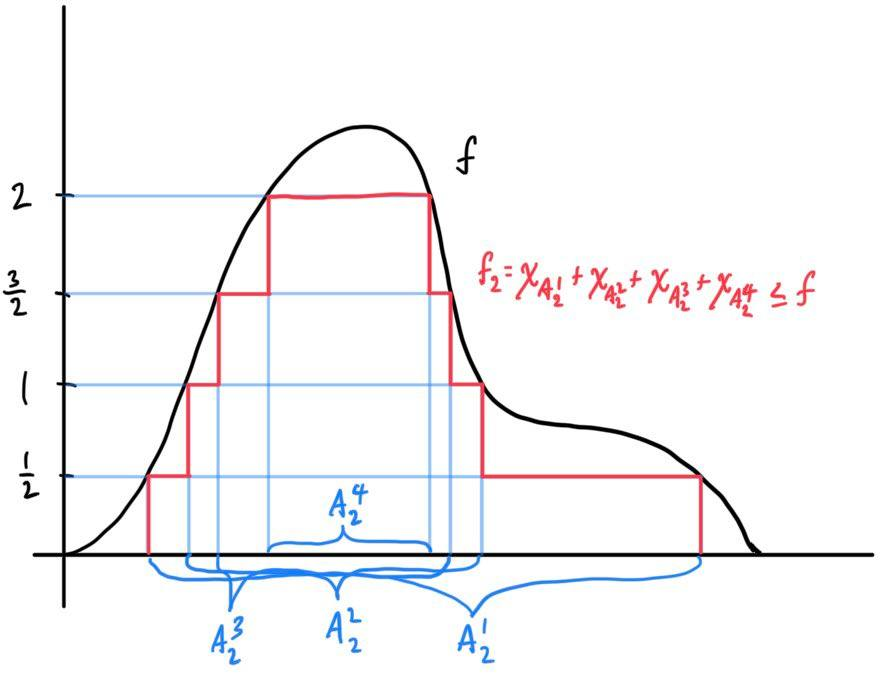
\includegraphics[scale=0.23]{img/Lebesgue_2.jpg}
      \end{center}
      and in general, we have $f_k = \sum_{j=1}^\infty \frac{1}{2^{k-1}} 1_{A^j_k}$. But we said a simple function is a \textit{finite} sum, and if $\infty$ is in the range of $f$, then this becomes a problem. We can quickly fix this by just truncating the summation at a certain point in the codomain ($f_1$ only considers intervals up to $1$, $f_2$ up to $2$ and so on), ultimately giving us 
      \begin{equation}
        f_k = \sum_{j=1}^{k 2^{k-1}} \frac{1}{2^{k-1}} 1_{A^j_k}
      \end{equation}
    \end{proof}

  \subsubsection{Lebesgue Integral}

    Finally, we can learn how to integrate. We require the positiveness condition on $f$ below because our previous theorem on approximating arbitrary functions with simple measurable functions $f_k$ requires that it be positive, too. 

    \begin{definition}[Lebesgue Integral of Positive Simple Functions]
      If $f = \sum_{k=1}^n c_k 1_{A_k}$ is a positive simple Lebesgue measurable function on measure space $(X, \mathcal{A}, \mu)$, then the \textbf{Lebesgue integral} of $f$ is 
      \begin{equation}
        \int f \, d\mu = \sum_{k=1}^n c_k \mu(A_k)
      \end{equation}
    \end{definition}

    This Lebesgue integral agrees with the Riemann integral for step functions. Let $c_1, \ldots, c_n \in [0, \infty)$ and $a = x_0 < x_1 < \ldots < x_n = b$ be a partition. Let $f: [a, b] \longrightarrow [0, \infty]$ be a step function taking the value $c_i$ on the interval $(x_{i-1}, x_i)$ for $i = 1, \ldots, n$. Then the Riemann integral of $f$ is simply 
    \begin{equation}
      \int f(x) \,dx = \sum_{i=1}^n c_k |x_i - x_{i-1}|
    \end{equation}
    The Lebesgue integral is 
    \begin{align*}
      \int f \, d \mu & = \sum_{i=1}^n c_i \mu((x_{i-1}, x_i)) + \sum_{j=0}^n f(x_j) \mu(\{x_j\}) \\
      & = \sum_{i=1}^n c_k |x_i - x_{i-1}|
    \end{align*}
    which agrees with the Riemann integral. In the Riemann integral, we write $dx$ to indicate the variable that is being integrated over, but in the Lebesgue integral, we write $d \mu$, the measure which we are integrating over. Therefore, there are many possible values that can come out of a Lebesgue integral of a certain function, while a Riemann integral outputs only one value if exists. 

    \begin{example}
      Consider the simple function (consisting of one characteristic function) $1_{\mathbb{Q} \cap [0, 1]}$. $\mathbb{Q} \cap [0, 1]$ is a Lebesgue measurable set of $\mathbb{R}$, and we have $1_{\mathbb{Q} \cap [0, 1]} \geq 0$, so its Lebesgue integral is given by the above definition: 
      \begin{equation}
        \int_{\mathbb{R}} 1_{\mathbb{Q} \cap [0, 1]} \, d\lambda = 1 \cdot \lambda(\mathbb{Q} \cap [0, 1]) = 0
      \end{equation}
    \end{example}

    \begin{definition}[Lebesgue Integral on Positive Measurable Functions]
      If $f: (X, \mathcal{A}, \mu) \longrightarrow [0, \infty]$ is measurable, then 
      \begin{equation}
        \int_X f \, d\mu = \sup \Big\{ \int g\, d\mu \,\Big|\, g \text{ simple }, g \leq f\Big\}
      \end{equation}
    \end{definition}

    Unlike Riemann integration, which looks at both the supremum and infimum of integrals of simple functions, Lebesgue integration only looks at the supremum, given that $f$ is nonnegative, so for all these $f$, the Lebesgue integral always exists. Defining Lebesgue integration for all real-valued functions, requires a simple extension. 

    \begin{definition}[Lebesgue Integral]
    Given a function $f: (X, \mathcal{A}, \mu) \longrightarrow \mathbb{R}$, we can split $f$ into a positive and negative part: 
    \begin{equation}
      f = f^+ - f^-
    \end{equation}
    where $f^+ = \max(f, 0)$ and $f^- = \max(-f, 0)$. Then, the Lebesgue integral of $f$ is 
    \begin{equation}
      \int f \, d \mu = \int f^+ \, d\mu - \int f^- \, d\mu
    \end{equation}
    given that at least one of these integrals is finite. If one is infinite and the other is finite, then we can call it infinite. If we have \textit{both} infinite integrals, then the integral doesn't exist. It has the properties: 
    \begin{enumerate}
      \item Monotonicity: 
      \begin{equation}
        g \leq f \implies \int g \, d\mu \leq \int f\, d\mu
      \end{equation}
      \item Scalar Multiplication: 
      \begin{equation}
        \int c f \, d\mu = c \int f \, d\mu
      \end{equation}
      \item Addition:
      \begin{equation}
        \int f + g \, d\mu = \int f \,d\mu + \int g \,d\mu
      \end{equation}
    \end{enumerate}
    \end{definition}

    Since $|f| = f^+ + f^-$, $f$ is also Lebesgue integrable if 
    \begin{equation}
      \int |f| \, d\mu < \infty
    \end{equation}
    since by triangle inequality, we have 
    \begin{equation}
      \bigg| \int f \, d\mu \bigg| \leq \int |f| \, d \mu
    \end{equation}

    \begin{definition}
      The set of all functions $f: (X, \mathcal{A}, \mu) \longrightarrow \mathbb{R}$ that are Lebesgue integrable is denoted $\mathcal{L}^1(X, \mathcal{A}, \mu; \mathbb{R})$, or for short $\mathcal{L}^1(X, \mathcal{A}, \mu)$. 
    \end{definition}

    \begin{theorem}
      $f: \mathbb{R} \longrightarrow \mathbb{R}$ is Riemann integrable iff it is continuous $\lambda$ almost everywhere. If so, then $f$ is Lebesgue measurable and 
      \begin{equation}
        \int_{[a, b]} f \,d\lambda = \int_a^b f \, dx
      \end{equation}
      for all $a < b$. 
    \end{theorem}

  \subsubsection{Integral Inequalities}

    We introduce 3 important inequalities on the integral. 

    \begin{theorem}[Jensen's Inequality]
      Suppose $\phi$ is convex, that is, 
      \begin{equation}
        \lambda \phi(x) + (1 - \lambda) \phi(y) \geq \phi (\lambda x + (1 - \lambda) y)
      \end{equation}
      for all $\lambda \in (0, 1)$ and $x, y \in \mathbb{R}$. If $\mu$ is a probability measure, and $f$ and $\varphi(f)$ are integrable, then 
      \begin{equation}
        \varphi\bigg( \int f \,d\mu \bigg) \leq \int \varphi(f) \,d\mu
      \end{equation}
    \end{theorem}

    \begin{theorem}[Holder's Inequality]
      If $p, q$ are Holder conjugates, then 
      \begin{equation}
        \int |f g|\, d\mu \leq ||f||_p ||g||_q
      \end{equation}
    \end{theorem}

    \begin{corollary}[Cauchy-Schwarz Inequality]
      Given that $p = q = 2$ above, then we have 
      \begin{equation}
        \int |f g|\, d\mu \leq ||f||_2 ||g||_2
      \end{equation}
      which is similar to the familiar equation $\langle u, v \rangle \leq ||u|| ||v||$. 
    \end{corollary}

  \subsubsection{Convergence Theorems}

    Now, we want to give conditions that guarantee 
    \begin{equation}
      \lim_{n \rightarrow \infty} \int f_n \,d \mu = \int \big( \lim_{n \rightarrow \infty} f_n \big) \, d\mu
    \end{equation}

    \begin{definition}[Convergence in Measure]
      A sequence of functions $f_n \rightarrow f$ \textbf{in measure} if for any $\epsilon > 0$, 
      \begin{equation}
        \mu\big( \{x \,:\, |f_n (x) - f(x)| > \epsilon \}\big) \rightarrow 0 \text{ as } n \rightarrow \infty
      \end{equation}
    \end{definition}

    \begin{theorem}[Bounded Convergence Theorem]
      Let $E$ be a set with $\mu(E) < \infty$. Suppose $f_n = 0$ on $E^c$, $|f_n (x)| \leq M$, and $f_n \rightarrow f$ in measure. Then, 
      \begin{equation}
        \int f \,d\mu = \lim_{n \rightarrow \infty} \int f_n d\mu
      \end{equation}
    \end{theorem}

    \begin{lemma}[Fatou's Lemma]
      If $f_n \geq 0$, then
      \begin{equation}
        \lim_{n \rightarrow \infty} \inf \int f_n \,d\mu \geq \int \Big( \lim_{n \rightarrow \infty} \inf f_n \Big) \,d\mu
      \end{equation}
    \end{lemma}

    \begin{theorem}[Monotone Convergence Theorem]
      Given a nondecreasing sequence of measurable nonnegative functions $\{f_n\}$, its limit $f_n \uparrow f$ always exists (since $f_n$ is nondecreasing), is measurable, and 
      \begin{equation}
        \int f_n \, d\mu \uparrow \int f \, d\mu
      \end{equation}
      This allows us to integrate the limit of nice functions $f_n$ by integrating these $f_n$ first and then finding what the values converge to. 
    \end{theorem}

    \begin{theorem}[Dominated Convergence Theorem]
      If $f_n \rightarrow f$ a.e., $|f_n| \geq g$ for all $n$, and $g$ is integrable, then 
      \begin{equation}
        \int f_n \,d\mu \rightarrow \int f\, d\mu
      \end{equation}
    \end{theorem}

  \subsubsection{Product Measures, Fubini's Theorem}

    Let $(X, \mathcal{A}, \mu_1)$ and $(Y, \mathcal{B}, \mu_2)$ be two measure spaces. Let 
    \begin{align*}
      \Omega & = X \times Y = \{(x, y) \mid x \in X, y \in Y\} \\
      \mathcal{S} & = \{A \times B \mid A \in \mathcal{A}, B \in \mathcal{B}\}
    \end{align*}
    The sets in $\mathcal{S}$ are called \textbf{rectangles}. It is easy to see that $\mathcal{S}$ is a semi-algebra: 
    \begin{align*}
      (A \times B) \cap (C \times D) & = (A \cap C) \times (B \cap D) \\
      (A \times B)^c & = (A^c \times B) \cup (A \times B^c) \cup (A^c \times B^c) 
    \end{align*}

    \begin{theorem}
      There is a unique measure $\mu = \mu_1 \times \mu_2$ (or denoted $\mu_1 \otimes \mu_2$) on $\mathcal{F}$ with 
      \begin{equation}
        \mu(A \times B) = \mu_1 (A) \, \mu_2 (B)
      \end{equation}
    \end{theorem}

    \begin{theorem}[Fubini's Theorem]
      Let $(X, \mathcal{A}, \mu_1)$ and $(Y, \mathcal{B}, \mu_2)$ be two measure spaces and $(X \times Y, \mathcal{F}, \mu = \mu_1 \times \mu_2)$ be their product space. Then, if $f \geq 0$ or $\int_{X \times Y} |f| \,d\mu < \infty$, then 
      \begin{equation}
        \int_X \int_Y f(x, y) \, \mu_2 \mu_1 = \int_{X \times Y} f \,d\mu = \int_Y \int_X f(x, y) \, \mu_1 \mu_2
      \end{equation}
    \end{theorem}

\subsection{Random Vectors}

  Now when we consider several random variables, they will all be defined on the same probability space. Given two random variables $X$ and $Y$ on $(\Omega, \mathcal{F}, \mathbb{P})$, they will each induce a probability law $\mathbb{P}_X$ and $\mathbb{P}_Y$ which completely characterizes them. Note that it is the same underlying randomness that is feeding these random variables, and so if I know some information about the value of $X$, then we know something about outcome $\omega$, which can be used to find something about the value of $Y$. To capture this, we can imagine the map $(X, Y) : \Omega \longrightarrow \mathbb{R}^2$ defined $(X, Y)(\omega) \coloneqq (X(\omega), Y(\omega))$. And just like how $X$ induces a measure $P_X$ onto $\mathbb{R}$, we can imagine $(X, Y)$ inducing a measure onto $\mathcal{B}(\mathbb{R}^2)$, which can be generated by all semi-infinite rectangles $(-\infty, x] \times (-\infty, y]$. Ideally, we would want to put a measure $\mathbb{P}_{X, Y}$ on $\mathbb{R}^2$ s.t. 
  \begin{equation}
    \mathbb{P}_{X, Y}(B) \coloneqq \mathbb{P}((X, Y)^{-1}(B))
  \end{equation}
  where $(x, y)^{-1}(b) = \{ \omega \in \omega \mid (x(\omega), y(\omega)) \in b\}$ denotes the preimage of $(x, y)$. but is $(x, y)^{-1}(b)$ $\mathcal{f}$-measurable? it turns out that it is. 

  \begin{theorem}
    Let $f: (X, \mathcal{A}, \mu) \longrightarrow \mathbb{R}^n$ have component functions $f_1, f_2, \ldots, f_n$. Then, $f$ is measurable (i.e. $f^{-1} (B) \in \mathcal{A}$ for all $B \in \mathcal{B}(\mathbb{R}^n)$) if and only if all of its component functions are measurable (i.e. $f_i^{-1} (B) \in \mathcal{A}$ for all $B \in \mathcal{B}(\mathbb{R}^n)$). 
  \end{theorem}

  From the theorem above, I have a probability law $\mathbb{P}_{X, Y}$ on all Borel sets of $\mathbb{R}^2$, making $(\mathbb{R}^2, \mathcal{B}(\mathbb{R}^2), \mathbb{P}_{X, Y})$ a probability space. Now, since $X$ and $Y$ are both random variables dependent on the same $\omega \in \Omega$, we could expect certain "combinations" of $X$ and $Y$ to be more probable than other combinations. 

  \begin{definition}[Joint Probability Law]
    Given two random variables $X, Y$ on $(\Omega, \mathcal{F}, \mathbb{P})$, the \textbf{joint random variable} $(X, Y): \Omega \longrightarrow \mathbb{R}^2$ is a measurable function defined 
    \begin{equation}
      (X, Y) (\omega) \coloneqq (X(\omega), Y(\omega))
    \end{equation}
    which induces a \textbf{joint probability law} $\mathbb{P}_{X, Y}: \mathcal{B}(\mathbb{R}^2) \longrightarrow [0, 1]$ defined 
    \begin{equation}
      \mathbb{P}_{X, Y}(B) \coloneqq \mathbb{P}((X, Y)^{-1}(B)) \; \forall B \in \mathcal{R}
    \end{equation}
    of $X, Y$. This law captures everything there is about the interdependence of $X$ and $Y$. 
  \end{definition}

  Given joint probability law $\mathbb{P}_{X, Y}$, we can get the probability laws of $X$ and $Y$ separately. For example, we can take a specific Borel set of $\mathbb{R}$ representing the outcomes of $X$ and look at every single combination of it with every $Y$. But knowing $\mathbb{P}_X$ and $\mathbb{P}_Y$ is not enough to know the joint $\mathbb{P}_{X, Y}$. 

  \begin{definition}[Marginal Probability Law]
    Given a joint probability law $\mathbb{P}_{X, Y}$ of $X, Y$, we can get the \textbf{marginal probability law} of $X$ by feeding in Borel sets of form $B \times \mathbb{R} \in \mathcal{B}(\mathbb{R}^2)$. 
    \begin{equation}
      \mathbb{P}_X (B) = \mathbb{P}_{X, Y} (B \times \mathbb{R})
    \end{equation}
    and the marginal probability law of $Y$ as 
    \begin{equation}
      \mathbb{P}_Y (B) = \mathbb{P}_{X, Y} (\mathbb{R} \times B)
    \end{equation}
  \end{definition}

  \begin{definition}[Joint Cumulative Distribution Function]
    Since sets of the form $(-\infty, x] \times (-\infty, y]$ are Borel in $\mathbb{R}^2$, the \textbf{joint cumulative distribution function} 
    \begin{align*}
      F_{X, Y} & \coloneqq \mathbb{P}_{X, Y} \big( (-\infty, x] \times (-\infty, y] \big) \\
      & = \mathbb{P} \big( \{\omega \mid X(\omega) \leq x\} \cap \{ \omega \mid Y(\omega) \leq y\} \big)
    \end{align*}
    is well-defined. By abuse of notation, we will write $F_{X, Y} (x, y) = \mathbb{P}(X \leq x, Y \leq y)$. The marginal CDFs are defined 
    \begin{align*}
      F_X (x) & \coloneqq \mathbb{P}_{X, Y} ((-\infty, x) \times \mathbb{R}) \\
      F_Y (y) & \coloneqq \mathbb{P}_{X, Y} (\mathbb{R} \times (-\infty, y))
    \end{align*}
  \end{definition}

  \begin{lemma}[Properties of Joint CDF]
    Some common properties of the joint CDF are as follows: 
    \begin{enumerate}
      \item Limits. 
      \begin{equation}
        \lim_{(x, y) \rightarrow (+\infty, +\infty)} F_{X, Y} (x, y) = 1 \text{ and } \lim_{(x, y) \rightarrow (-\infty, -\infty)} F_{X, Y} (x, y) = 0
      \end{equation}
      \item Monotonicity. 
      \begin{equation}
        x_1 \leq x_2, \; y_1 \leq y_2 \implies F_{X, Y} (x_1, y_1) \leq F_{X, Y}(x_2, y_2)
      \end{equation}
      \item Continuity from above. 
      \begin{equation}
        \lim_{\epsilon \rightarrow 0^+} F_{X, Y} (x + \epsilon, y + \epsilon) = F_{X, Y} (x, y) \text{ for all } x, y \in \mathbb{R}
      \end{equation}
      \item Maringal CDFs. 
      \begin{equation}
        \lim_{y \rightarrow \infty} F_{X, Y} (x, y) = F_X (x), \;\;\;\; \lim_{x \rightarrow \infty} F_{X, Y} (x, y) = F_Y (y)
      \end{equation}
    \end{enumerate}
  \end{lemma}

  \subsubsection{Joint Discrete Random Variables}

    \begin{definition}[Joint PMF]
      Given discrete random variables $X$ and $Y$, let their countable images be denoted $E_X, E_Y \subset \mathbb{R}$. Then, $E_X \times E_Y$ is also countable, and so the joint random variable $(X, Y)$ is also discrete. This means that we can write for some Borel $B$ of $\mathbb{R}^2$, 
      \begin{equation}
        \mathbb{P}_{X, Y} (B) = \sum_{(x, y) \in (E_X \times E_Y) \cap B} \mathbb{P}_{X, Y} (\{(x, y)\})
      \end{equation}
      and we can define the PMF as $p_{X, Y} (x, y) \coloneqq \mathbb{P}_{X, Y} (\{(x, y)\})$. By abuse of notation, we write $p_{X, Y} (x, y) = \mathbb{P} (X = x, Y = y)$ and write 
      \begin{equation}
        \mathbb{P}_{X, Y} (B) = \sum_{(x, y) \in (E_X \times E_Y) \cap B} \mathbb{P} (X = x, Y = y)
      \end{equation}
      If you give me a joint PMF $p_{X, Y}$, by the definition above this determines the entire probability law of $\mathbb{P}_{X, Y}$. 
    \end{definition} 

    \begin{definition}[Conditional PMF]
      Let $X, Y$ be discrete random variables on $(\Omega, \mathcal{F}, \mathbb{P})$. The \textbf{conditional PMF} of $X$ given $Y = y$ is defined 
      \begin{equation}
        p_{X \mid Y} (x \mid y) \coloneqq \frac{p_{X, Y} (x, y)}{p_Y (y)} = \frac{\mathbb{P}_{X, Y} (\{x, y\})}{\mathbb{P}_Y (\{y\})}
      \end{equation}
      and again by abuse of notation, we can simply write 
      \begin{equation}
        \mathbb{P}(X = x \mid Y = y) \coloneqq \frac{\mathbb{P}(X = x, Y = y)}{\mathbb{P}(Y = y)}
      \end{equation}
    \end{definition}

    \begin{theorem}[TFAE]
      Let $X$ and $Y$ be discrete random variables. Then, the following are equivalent: 
      \begin{enumerate}
        \item $X$ and $Y$ are independent. 
        \item For all $x, y \in \mathbb{R}$, the events $\{X = x\}$ (aka $X^{-1} (\{x\})$) and $\{Y = y\}$ (aka $Y^{-1} (\{y\})$) are independent. That is, 
        \begin{equation}
          \mathbb{P} \big[ X^{-1}(\{x\}) \cap Y^{-1}(\{y\}) \big] = \mathbb{P}(X^{-1}(\{x\})) \, \mathbb{P}(Y^{-1}(\{y\}))
        \end{equation}
        \item For all $x, y \in \mathbb{R}$, $p_{X, Y} (x, y) = p_X (x) \cdot p_Y (y)$. 
        \item For all $x, y \in \mathbb{R}$ such that $p_Y (y) > 0$, we have $p_{X \mid Y}(x \mid y) = p_X (x)$. 
      \end{enumerate}
    \end{theorem}

  \subsubsection{Joint Continuous Random Variables}

    \begin{definition}
      $X$ and $Y$ are jointly continuous if the joint law $\mathbb{P}_{X, Y}$ is absolutely continuous w.r.t. the Lebesgue measure on $\mathbb{R}^2$ (i.e. a Borel set of Lebesgue measure $0$ must have $P_{X, Y} = 0$ also). 
    \end{definition}

    However, $X$ and $Y$ continuous does not always imply that $(X, Y)$ are jointly continuous! If we have $X \sim \mathcal{N}(0, 1)$ and $Y = 2 X \sim \mathcal{N}(0, 4)$. Jointly continuous allows us to define a PDF on it. 

    \begin{theorem}[Radon-Nikodym Theorem]
      If $X$ and $Y$ are jointly continuous RVs, then there exists a measurable $f_{X, Y} : \mathbb{R}^2 \longrightarrow [0, \infty)$ s.t. for any $B \in \mathcal{B}(\mathbb{R}^2)$, we have 
      \begin{equation}
        \mathbb{P}_{X, Y} (B) = \int_B f_{X, Y} \, d\lambda
      \end{equation}
    \end{theorem}

    The Radon-Nikodym Theorem guarantees the existence of such $f_{X, Y}$. Taking $B = (-\infty, x] \times (-\infty, y]$, we can define the joint CDF as 
    \begin{equation}
      F_{X, Y} (x, y) = \mathbb{P}(X \leq x, Y \leq y) \coloneqq \mathbb{P}_{X, Y} \big( (-\infty, x] \times (-\infty, y] \bigg) = \int_{-\infty}^x \int_{-\infty}^y f_{X, Y} (s, t) \, dt \,ds
    \end{equation}

\subsection{Expectation}

  \begin{definition}[Expectation]
    Given a probability space $(\Omega, \mathcal{F}, \mathbb{P})$ and a random variable $X: \Omega \longrightarrow \mathbb{R}$, the \textbf{expectation} of $X$ is defined 
    \begin{equation}
      \mathbb{E}[X] \coloneqq \int_\Omega X \, d\mathbb{P}
    \end{equation}
    Generally, if we are integrating over the entire probability space, then it is conventional to not write $\Omega$ in the integral at all: $\mathbb{E}[X] = \int X \,d\mathbb{P}$. 
  \end{definition}

  \begin{definition}[Expectation of Discrete RV]
    If $X$ is a discrete random variable \textit{that takes positive values}, then let $E = \{e_1, e_2, \ldots\}$ denote the set where $\mathbb{P}_X(E) = 1$, and let $E_i = X^{-1} (\{e_i\}) \subset \Omega$. Then, we can see that since $X$ is constantly $e_i$ on $E_i$, 
    \begin{equation}
      \int_{E_i} X \, d\mathbb{P} = e_i \cdot \mathbb{P}(E_i) = e_i \cdot \mathbb{P}_X (\{e_i\}) = e_i \cdot \mathbb{P}(X = e_i)
    \end{equation}
    which implies 
    \begin{equation}
      \mathbb{E}[X] = \int_\Omega X \, d\mathbb{P} = \sum_{i=1}^\infty \int_{E_i} X \, d\mathbb{P} = \sum_{i=1}^\infty e_i \cdot \mathbb{P}(X = e_i)
    \end{equation}
    If $X$ is discrete RV possibly taking negative values, then let $X = X^+ - X^-$, where $X^+ = \max(X, 0)$ and $X^- = - \min(X, 0)$. Then, we can compute 
    \begin{equation}
      \mathbb{E}[X] = \mathbb{E}[X^+] - \mathbb{E}[X^-]
    \end{equation}
    which is well-defined as long as we don't have "$\infty - \infty$."
  \end{definition}

  Note that the reason why expectations of the form $\infty - \infty$ are indeterminate is because of the Riemann rearrangement theorem. 

  \begin{theorem}[Riemann's Rearragenement Theorem]
    Given a series $\sum a_n$ that is conditionally convergent (i.e. converges but not absolutely convergent), the terms can be arranged so that the new series converges to an arbitrary real number, or diverges. 
  \end{theorem}

  \begin{lemma}[Properties of Expectation]
    Let $X$ and $Y$ be random variables with finite expectations. 
    \begin{enumerate}
      \item Monotonicity: If $X \leq Y$ (i.e. $X(\omega) \leq Y(\omega)$ for all $\omega \in \Omega$), then 
      \begin{equation}
        \mathbb{E}[X] \geq \mathbb{E}[Y]
      \end{equation}
      
      \item Non-Negativity: This is implied from the above if we set the lower bound to the constant random variable $0$. If $X \geq 0$, then 
      \begin{equation}
        \mathbb{E}[X] \geq 0
      \end{equation}
      
      \item Linearity: For all $a, b, c \in \mathbb{R}$, 
      \begin{equation}
        \mathbb{E}[a X + b Y + c] = a \mathbb{E}[X] + b \mathbb{E}[Y] + c
      \end{equation}
    \end{enumerate}
  \end{lemma}

  We now show a widely-used, but nontrivial, theorem. 

  \begin{theorem}[Expectation of Independent Events]
    Given independent RVs $X$ and $Y$, 
    \begin{equation}
      \mathbb{E}[X Y] = \mathbb{E}[X] \, \mathbb{E}[Y]
    \end{equation}
  \end{theorem}
  \begin{proof}
    We show only for simple random variables which will give us a start in proving for all random variables in full generality. Let $X$ and $Y$ be simple random variables, i.e. 
    \begin{equation}
      X = \sum_i a_i 1_{A_i} \text{ and } Y = \sum_j b_j 1_{B_j}
    \end{equation}
    Since $\{A_i\}_i$ and $\{B_j\}_j$ are both partitions, $\{A_i \cap B_j\}_{i, j}$ is also a partition, and 
    \begin{equation}
      X Y = \sum_{i, j} a_i b_j \, 1_{A_i \cap B_j}
    \end{equation}
    Its expectation can be expanded out by linearity, and since $\mathbb{E}[ 1_{A} ] = \mathbb{P}(A)$, we have
    \begin{align*}
      \mathbb{E}[X Y] & = \sum_{i, j} a_i b_j \, \mathbb{P}(A_i \cap B_j) \\
      & = \sum_{i, j} a_i b_j \, \mathbb{P}(A_i)\, \mathbb{P}(B_j) = \mathbb{E}[X] \, \mathbb{E}[Y]
    \end{align*}
    Now that we have proved for simple random variables, we can just approximate $X$ from below using simple functions. 
  \end{proof}

  \begin{theorem}[Tail Sum Formula]
    If a discrete random variable $X$ takes values in the non-negative integers $\{0, 1, 2, 3, ...\}$, then 
    \begin{equation}
      \mathbb{E}[X] = \sum_{k=1}^\infty \mathbb{P}(X \geq k)
    \end{equation}
    In any case (continuous or discrete), if $X$ is a non-negative random variable, then 
    \begin{equation}
      \mathbb{E}[X] = \int_0^\infty \mathbb{P}(X > x) \, dx = \int_0^\infty 1 - F(x) \, dx
    \end{equation}
    where $F$ is the CDF of $X$. 
  \end{theorem}
  \begin{proof}
    Suppose that $X$ takes values in $\{0, 1, 2, 3, ...\}$. Then, 
    \begin{align*}
      \mathbb{E}[X] & = \sum_{k \geq 1} k \, \mathbb{P}(X=k) \\
      & = \sum_{k\geq 1} \sum_{j=1}^k \mathbb{P}(X = k) \\
      & = \sum_{k \geq 1} \sum_{j=1}^k 1_{j \leq k} \, \mathbb{P}(X=k) \\
      & = \sum_{j=1}^\infty \sum_{k \geq 1} 1_{j \leq k} \, \mathbb{P}(X =k) \\
      & = \sum_{j=1}^\infty \sum_{k \geq j} \mathbb{P}(X=k) \\
      & = \sum_{j=1}^\infty \mathbb{P}(X \geq j)
    \end{align*}
  \end{proof}

  \begin{corollary}
    For any $m > 0$ and $\alpha > 0$,  
    \begin{equation}
      \mathbb{P} \big(|X| > \alpha \big) \leq \frac{1}{\alpha^m} \mathbb{E} \big( |X|^m \big)
    \end{equation}
  \end{corollary}

  \begin{example}[Geometric RV]
    Recall that given $X \sim \mathrm{Geometric}(p)$, we have $\mathbb{P}(X = i) = (1 - p)^{i-1} p$ for $i \geq 1$. So, 
    \begin{equation}
      \mathbb{E}[X] = \sum_{x=1}^\infty x \, \mathbb{P}(X = x) = \sum_{x=1}^\infty x \, (1 - p)^{i-1} p = \frac{p}{(1 - (1 - p))^2} = \frac{1}{p}
    \end{equation}
  \end{example}

  \begin{example}[Infinite Expectation]
    Let us have discrete random variable s.t. $\mathbb{P}(X = k) = \frac{6}{\pi^2} \frac{1}{k^2}$ for $k \geq 1$. So, 
    \begin{equation}
      \mathbb{E}[X] = \sum_{k=1}^\infty k \, \mathbb{P}(X = k) = \frac{6}{\pi^2} \sum_{k=1}^\infty \frac{1}{k} = +\infty
    \end{equation}
  \end{example}

  \begin{example}[Undefined Expectation]
    Let $\mathbb{P}(X = k) = \frac{3}{\pi^2} \frac{1}{k^2}$ for $k \in \mathbb{Z}\setminus \{0\}$. The expectation of this can be computed by getting the expectation of all the positive terms and the negative terms. 
    \begin{equation}
      \mathbb{E}[X] = \mathbb{E}[X^+] - \mathbb{E}[X^{-}] = \sum_{k=1}^\infty k \cdot \frac{3}{\pi^2} \frac{1}{k^2} + \sum_{k=1}^\infty (-k) \cdot \frac{3}{\pi^2} \frac{1}{k^2} = \infty - \infty
    \end{equation}
    Note that by the Riemann rearrangement theorem, we can't just say that the expectation is $0$ since the terms "cancel out." We could only do this if the series is absolutely convergent also, which works if $X$ takes positive values only. 
  \end{example}

  Note that when we compute expectation, what we do it multiply the PMF/PDF by $x$ and sum/integrate over it. The Cauchy distribution is a power function of form $\frac{1}{x^2}$, so if we multiply it by $x$, we have the new $\frac{1}{x}$ which is divergent. 

  \subsubsection{Law of the Unconscious Statistician}

    Given probability space $(\Omega, \mathcal{F}, \mathbb{P})$ and a random vector $X: \Omega \rightarrow \mathbb{R}^n$, this induces a probability law $\mathbb{P}_X$ acting as a measure on $\mathbb{R}^n$. Assume that this probability law $\mathbb{P}_X$ is known. Now introduce a function $g: \mathbb{R}^n \rightarrow \mathbb{R}$. We can create a new random variable $Y = g \circ X : \Omega \rightarrow \mathbb{R}$ with its own probability law $\mathbb{P}_Y$ on $\mathbb{R}$. Since we already know the probability distribution of $X$, so we can easily get the expected value of $X$ as (in the discrete case) 
    \begin{equation}
      \mathbb{E}[X] = \sum_{x \in \mathcal{X}} x \cdot \mathbb{P}(X = x)
    \end{equation}
    where $\mathcal{X}$ is the support of $X$. But what if we wanted to get the expected value of $Y$? 
    \begin{equation}
      \mathbb{E}[Y] = \sum_{y \in \mathcal{Y}} y \cdot \mathbb{P}(Y = y) = ?
    \end{equation}
    The problem is that we don't know the probability distribution of $Y$. But since we know that all the values of $X$ are transformed by $g$, we are taught to compute it in terms of the probability distribution of $X$. 
    \begin{equation}
      \mathbb{E}[Y] = \sum_{x \in \mathcal{X}} g(x) \cdot \mathbb{P}(X = x)
    \end{equation}
    This "identity" that is often used must actually be treated as a rigorous theorem. This is like a change of basis formula that allows us to shift to a convenient space to compute integrals. 

    \begin{theorem}[LOTUS]
      Given probability space $(\Omega, \mathcal{F}, \mathbb{P})$, a random variable $X: \Omega \rightarrow \mathbb{R}^n$, and a function $g: \mathbb{R}^n \rightarrow \mathbb{R}$, the expectation of $g(X)$ is 
      \begin{equation}
        \mathbb{E}[g(X)] = \int_\Omega g(X) \,d\mathbb{P} = \int_{\mathbb{R}^n} g \, d\mathbb{P}_X = \int_\mathbb{R} \,d \mathbb{P}_{g(X)}
      \end{equation}
      It is usually the case that we don't know the distribution of $g(X)$ since $g$ is too complicated (hard to compute the right integral) and we don't want to integrate over an abstract space $\Omega$ where we can't do calculus on (hard to compute the left integral). But we do know the distribution of $X$, so we can indeed compute the middle integral. 
    \end{theorem}

    Note that if $g: \mathbb{R} \rightarrow \mathbb{R}$ is the identity function $\mathrm{id}$, then we have 
    \begin{equation}
      \mathbb{E}[X] = \int_\Omega X \,d\mathbb{P} = \int_{\mathbb{R}} \mathrm{id} \, d\mathbb{P}_X
    \end{equation}
    \begin{enumerate}
      \item For the discrete case, the above integral simplifies to 
      \begin{equation}
        \mathbb{E}[g(X)] = \int_{\mathbb{R}^n} g \,d \mathbb{P}_X = \sum_{x \in \mathcal{X} \subset \mathbb{R}^n} g(x) p_X (x)
      \end{equation}
      
      \item For the continuous case, we have 
      \begin{equation}
        \mathbb{E}[g(X)] = \int_{\mathbb{R}^n} g \,d \mathbb{P}_X = \int_{\mathbb{R}^n} g (x) \, f_X (x) \,dx
      \end{equation}
    \end{enumerate}

  \subsubsection{Expectation w.r.t. Different Measures}

    Sometimes, we just write the expectation of a measurable function $f: (S, \mathcal{S}) \rightarrow \mathbb{R}$ as $\mathbb{E}[f]$. If we need to specify with respect to what measure we are integrating over, we write 
    \begin{equation}
      \mathbb{E}_\mu [f] \coloneqq \int_S f \, d\mu
    \end{equation}
    Usually, if $f$ represents some transformation of a random variable $X: \Omega \rightarrow S$, then we assume that we are integrating w.r.t. the probability measure $\mathbb{P}$ defined on $\Omega$ or the probability law $\mathbb{P}_X$ induced by $X$. 
    \begin{equation}
      \mathbb{E}[f] = \mathbb{E}[f(X)] = \int_\Omega f(X) \,d\mathbb{P} = \int_S f \,d\mathbb{P}_X
    \end{equation}

    \begin{example}[Expectation of Exponential RV]
    The PDF of exponential random variable $X$ is defined $f_X = k e^{-k x}$ for $x \geq 0$. So, 
    \begin{equation}
      \mathbb{E}[X] = \int_\mathbb{R} x f_X \, d\lambda = \int_0^\infty x k e^{-k x} \, dx = \frac{1}{k}
    \end{equation}
    Similarly, if we want the expectation of $X^2$, then we can get 
    \begin{equation}
      \mathbb{E}[X^2] = \int_\mathbb{R} x^2 f_X \,d\lambda = \int_0^\infty x^2 k e^{-k x} \,dx = \frac{2}{k^2}
    \end{equation}
    \end{example} 

    \begin{example}[Expectation of Gaussian RV]
      The expectation of a Gaussian random variable $X$ is
      \begin{equation}
        \mathbb{E}[X] = \int_{-\infty}^\infty x \cdot \frac{1}{\sigma \sqrt{2\pi}} e^{-\frac{(x - \mu)^2}{2 \sigma^2}} \, dx = \mu
      \end{equation}
    \end{example}

    \begin{example}[Expectation of One-Sided Cauchy]
      If we have $f_X (x) = \frac{2}{\pi} \frac{1}{1 + x^2}$ for $x \geq 0$, then 
      \begin{equation}
        \mathbb{E}[X] = \int_0^\infty \frac{2}{\pi} \frac{x}{1 + x^2} \,dx
      \end{equation}
      and making the substitution $t = \frac{1 + x^2}, \; dt = 2x$, we have 
      \begin{equation}
        \int_1^\infty \frac{1}{\pi} \frac{1}{t} \,dt = \frac{\ln(t)}{\pi} \bigg|_1^\infty = +\infty
      \end{equation}
    \end{example}

    \begin{example}[Expectation of Two-Sided Cauchy]
      The two-sided Cauchy is just another copy of the one sided into the negatives, so $f_X (x) = \frac{1}{\pi} \frac{1}{1 + x^2}$ for $x \in \mathbb{R}$. The expectation of $X$ should be split up into for positive and negative images, but computing it gives 
      \begin{equation}
        \mathbb{E}[X] = \mathbb{E}[X^+] - \mathbb{E}[X^-] = \int_0^\infty \frac{1}{\pi} \frac{x}{1 + x^2}\,dx - \int_{-\infty}^0 \frac{1}{\pi} \frac{x}{1 + x^2}\,dx = \infty - \infty
      \end{equation}
      and so it is undefined. 
    \end{example}

    With LOTUS, we can make sense of an extremely important inequality. 

    \begin{theorem}[Jensen's Inequality]
      If $f$ is a convex function, then $\mathbb{E}[f(X)] \geq f (\mathbb{E}[X])$. 
    \end{theorem}
    \begin{proof}
      We will assume that $f$ is differentiable for simplicity and let $\mathbb{E}[X] = \mu$. Define the linear function centered at $\mu$ to be $l(x) \coloneqq f(\mu) + f^\prime (\mu) (x - \mu)$. Then, we know that $f(x) \geq l(x)$ for all $x$, so 
      \begin{align*}
        \mathbb{E}[f(X)] & \geq \mathbb{E}[ l(X)] \\ 
        & = \mathbb{E}[f(\mu) + f^\prime (\mu) \, (X - \mu)] \\
        & = \mathbb{E}[f(\mu)] + f^\prime (\mu) ( \mathbb{E}[X] - \mu) \\
        & = \mathbb{E}[f(\mu)] \\
        & = f(\mathbb{E}[X])
      \end{align*}
    \end{proof}

    A nice way to visualize which side is greater (which I tend to always forget) is to think about a Bernoulli($p$) distribution. $f(\mathbb{E}[X])$ is visualized to be lower than the region in which the $\mathbb{E}[f(X)]$ must lie. 

    \begin{figure}[H]
      \centering 
      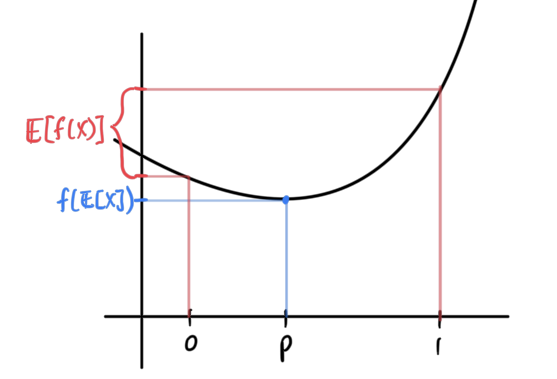
\includegraphics[scale=0.4]{img/jensen_visual.png}
      \caption{The function $f$ essentially transforms the Bernoulli defined on $0, 1$ to the Bernoulli defined on $f(0), f(1)$. Therefore, $\mathbb{E}[f(X)] \in [f(0), f(1)]$, which lies completely over $f(\mathbb{E}[X])$.} 
      \label{fig:jensen_visual}
    \end{figure}

\subsection{Variance, Covariance, Correlation}

  \begin{definition}[Variance]
    Let $X$ be a random variable and suppose $\mathbb{E}[X] < \infty$. The \textbf{variance} of $X$ is defined 
    \begin{equation}
      \mathrm{Var}[X] = \sigma^2_X \coloneqq \mathbb{E} [ (X - \mathbb{E}[X])^2 ]
    \end{equation}
    and $\sigma_X = \sqrt{\mathrm{Var}[X]}$ is called the \textbf{standard deviation}. This is a measure of how much the probability distribution deviates from its mean. We can use linearity of expectation to write 
    \begin{align*}
      \mathrm{Var}[X] & = \mathbb{E} \big[ X^2 + \mathbb{E}[X]^2 - 2 X \mathbb{E}[X] \big] \\
      & = \mathbb{E}[X^2] + \mathbb{E}[X]^2 - 2 \mathbb{E}[X] \mathbb{E}[X] \\
      & = \mathbb{E}[X^2] - \mathbb{E}[X]^2
    \end{align*}
    which is often easier to compute, since it only requires us to compute the expectation of $X$ and $X^2$. Since variance is always nonnegative, we also know that $\mathbb{E}[X^2] \geq \mathbb{E}[X]^2$. The variance is always defined, whether it's finite or $+\infty$. 
  \end{definition}

  Likewise for expectation, the variance of a function $f$ w.r.t. $\mu$ is 
  \begin{equation}
    \Var_\mu (f) = \mathbb{E}_\mu [f^2] - \mathbb{E}_\mu [f]^2
  \end{equation}

  \begin{proposition}
    The variance of a random variable $X$ is $0$ if and only if it constant almost everywhere on $\Omega$. 
  \end{proposition}
  \begin{proof}
    The if part is easy, so let's prove the only if part. Let $\mathbb{E} [ (X - \mathbb{E}[X])^2 ] = 0$. Then, we can think of the function $x \mapsto (x - \mathbb{E}[X])^2$ and write the variance as 
    \begin{equation}
      \mathrm{Var}[X] = \int_\Omega (X - \mathbb{E}[X])^2 \, d\mathbb{P} = 0
    \end{equation}
    But by nonnegativity of the function, we know that $(X - \mathbb{E}[X])^2 = 0$ w/ probability $1$, which implies that $X = \mathbb{E}[X]$ with prob. $1$. 
  \end{proof}

  \begin{lemma}[Properties of Variance]
    Let $X$ and $Y$ be random variables with well-defined variances. 
    \begin{enumerate}
      \item Translation Invariance: Given that $X + a$ is a new random variable defined $(X + a)(\omega) = X(\omega) + a$, 
      \begin{equation}
        \mathrm{Var}[X] = \mathrm{Var}[X + a]
      \end{equation}
      \item Quadratic Scaling: Given that $aX$ is a new random variable defined $(aX)(\omega) = a\,X(\omega)$, 
      \begin{equation}
        \mathrm{Var}[aX] = a^2 \mathrm{Var}[X]
      \end{equation}
    \end{enumerate}
  \end{lemma}

  From the properties of expectation and variance, we can now \textbf{standardize} a random variable $X$. If $X$ is a random variable with mean $\mu = \mathbb{E}[X]$ and variance $\sigma^2 = \Var(X)$, then the random variable 
  \begin{equation}
    Y = \frac{X - \mu}{\sigma}
  \end{equation}
  has mean $\mathbb{E}(Y) = 0$ and variance $\Var(Y) = 1$. 

  \begin{example}[Bernoulli]
    Given $X \sim \mathrm{Bernoulli}(p)$, we have
    \begin{align*}
      \mathbb{E}[X] & = 0 \cdot \mathbb{P}(X = 0) + 1 \cdot \mathbb{P}(X = 1) = p \\
      \mathbb{E}[X^2] & =  0^2 \cdot \mathbb{P}(X = 0) + 1^2 \cdot \mathbb{P}(X = 1) = p
    \end{align*}
    and so $\mathrm{Var}[X] = p - p^2 = p(1 - p)$. 
  \end{example}

  \begin{example}[Poisson]
    Given $X \sim \mathrm{Poisson}(X)$, then 
    \begin{align*}
      \mathbb{E}[X] & = \sum_{k = 0}^\infty k \cdot \frac{e^{-\lambda} \lambda^k}{k!} = \sum_{k = 1}^\infty \cdot \frac{e^{-\lambda} \lambda^k}{(k-1)!} = \lambda \sum_{k = 1}^\infty \cdot \frac{e^{-\lambda} \lambda^{k-1}}{(k-1)!} = \lambda\\
      \mathbb{E}[X] & = \sum_{k=0}^\infty k^2 \cdot \frac{e^{-\lambda} \lambda^k}{k!} = \ldots = \lambda^2 + \lambda
    \end{align*}
    So $\mathrm{Var}[X] = \lambda^2 + \lambda - \lambda^2 = \lambda$. 
  \end{example}

  \begin{example}[Uniform]
    Let $X \sim \mathrm{Uniform}[a, b]$. Then, 
    \begin{align*}
      \mathbb{E}[X] & = \int_\mathbb{R} x f_X \, d\lambda = \int_a^b x \cdot \frac{1}{b - a}\,dx = \frac{a + b}{2} \\
      \mathbb{E}[X^2] & = \int_\mathbb{R} x^2 f_X \,d\lambda = \int_a^b \frac{x^2}{b - a} \,dx = \frac{a^2 + ab + b^2}{3} 
    \end{align*}
    So $\mathrm{Var}[X] = \ldots = \frac{1}{12} (b - a)^2$. This is consistent with the fact that if we spread out our measure over a wider interval, then the variance will be bigger. 
  \end{example}

  \begin{example}[Exponential]
    Let $X \sim \mathrm{Exp}(\lambda)$. Then, $\mathbb{E}[X] = \frac{1}{\lambda}$ and $\mathbb{E}[X^2] = \frac{2}{\lambda^2}$, so 
    \begin{equation}
      \mathrm{Var}[X] = \frac{1}{\lambda^2}
    \end{equation}
    This is consistent with the fact that if $\lambda$ is greater, then the PDF is much more concentrated at $0$, making the variance small. 
  \end{example}

  Just like how we explained that computing finiteness or infiniteness of expectation is similar to multiplying the PMF/PDF by $x$ and determining if the series/integral converges or diverges, we can do the same for variance by multiplying the PMF/PDF by $x^2$. For a probability distribution of form $\frac{1}{x^2}$, it diverges if we multiply by $x$ and also diverges if we multiply by $x^2$. But also, we could construct a distribution where the expectation may be finite, but the variance may be infinite. For example, if we have a distribution of form $\frac{1}{x^3}$, multiplying it by $x$ leads to form $\frac{1}{x^2}$, which is finite (so finite expectation), but multiplying by $x^2$ leads to a harmonic, i.e. infinite variance. 

  \begin{definition}[Moment]
    The \textbf{$\mathbf{n}$th (raw) moment} of a random variable $X$ is $\mathbb{E}[X^n]$. Unlike the raw moment, which is calculated around the origin, the \textbf{$\mathbf{n}$th central moment} of $X$ is its moment centered around its mean $\mathbb{E}[(X - \mathbb{E}[X])^n]$. 
    \begin{enumerate}
      \item the first moment is the mean $\mathbb{E}[X]$
      \item the second central moment is the variance $\mathbb{E}[(X - \mathbb{E}[X])^2]$ 
      \item the third central moment, divided by $\sigma^3$, is the skew $\frac{1}{\sigma^3} \mathbb{E}[(X - \mathbb{E}[X])^3]$ 
    \end{enumerate}
  \end{definition}

  The variance is a measure for one random variable $X$, which measures how much it deviates from its mean. Now, the covariance is defined for two random variables and captures how they jointly vary. 

  \begin{definition}[Covariance]
    The \textbf{covariance} of random variables $X$ and $Y$ is defined as 
    \begin{align*}
      \mathrm{Cov}[X, Y] & = \mathbb{E} \big[ (X - \mathbb{E}[X]) (Y - \mathbb{E}[X]) \big] \\
      & = \mathbb{E}[X Y] - \mathbb{E}[X] \, \mathbb{E}[Y]
    \end{align*}
    where the intermediate expectations are well-defined. $X$ and $Y$ are said to be \textbf{uncorrelated} if 
    \begin{equation}
      \mathrm{Cov}[X, Y] = 0
    \end{equation}
  \end{definition}

  The covariance is also easy to interpret. Given two random variables $X$ and $Y$, if whenever $X$ is greater than its expected value $\mathbb{E}[X]$, $Y$ also tends to be greater than $\mathbb{E}[Y]$, then the covariance will be some positive number. If they tend to be on opposite sides of their expected values, then the covariance will be negative. And the degree with which these RVs lie on which side of the expected value determines the magnitude of the covariance. 

  \begin{theorem}
    If $X$ and $Y$ are independent random variables, then they are uncorrelated, meaning that independence is a stronger condition. 
  \end{theorem}

  We show an example of why the converse is not true. Consider $X \sim \mathrm{Uniform}[-1, 1]$. We can show that $x$ and $Y = X^2$ are dependent but uncorrelated. It is clearly dependent, but its covariance is 
  \begin{align*}
    \mathrm{Cov}(X, Y) & = \mathbb{E}[X Y] - \mathbb{E}[X] \, \mathbb{E}[Y] \\
    & = \mathbb{E}[X^3] - \mathbb{E}[X] \, \mathbb{E}[X^2] \\
    & = \int_{-1}^1 x^3 \cdot 1 \,dx - 0 \cdot \mathbb{E}[X^2] = 0
  \end{align*}

  \begin{theorem}[Variance of Sums of Random Variables]
    If $X$ and $Y$ are two random variables, then 
    \begin{equation}
      \mathrm{Var}(X + Y) = \mathrm{Var}[X] + \mathrm{Var}(Y) + 2 \mathrm{Cov}(X, Y)
    \end{equation}
    and by induction, we can show that 
    \begin{equation}
      \mathrm{Var}\bigg( \sum_i X_i\bigg) = \sum_{i} \mathrm{Var}(X_i) + \sum_{i, j} \mathrm{Cov}(X_i, X_j)
    \end{equation}
  \end{theorem}
  \begin{proof}
    Simple computation. The LHS expands to 
    \begin{align*}
      \mathbb{E}[(X + Y)^2] - \mathbb{E}[X + Y]^2 & = \mathbb{E}[X^2 + 2XY + Y^2] - (\mathbb{E}[X] + \mathbb{E}[Y])^2 \\
      & = \mathbb{E}[X^2] + 2 \mathbb{E}[XY] + \mathbb{E}[Y^2] - \mathbb{E}[X]^2 - 2 \mathbb{E}[X] \mathbb{E}[Y] - \mathbb{E}[Y]^2 \\
      & = \big( \mathbb{E}[X^2] - \mathbb{E}[X]^2 \big) + \big( \mathbb{E}[Y^2] - \mathbb{E}[Y]^2 \big) + 2 \big( \mathbb{E}[XY] - \mathbb{E}[X] \mathbb{E}[Y] \big) \\
      & = \mathrm{Var}[X] + \mathrm{Var}(Y) + 2 \mathrm{Cov}(X, Y) 
    \end{align*}
  \end{proof}

  Therefore, if we have $n$ random variables $X_1, \ldots, X_n$, then we can compute their pairwise covariance $\mathrm{Cov}(X_i, X_j)$ and compute their \textbf{covariance matrix} $\boldsymbol{\Sigma}$, which is an $n \times n$ symmetric matrix with entries 
  \begin{equation}
    \boldsymbol{\Sigma}_{ij} = \mathrm{Cov}(X_i, X_j) \text{ for } i, j = 1, \ldots, n
  \end{equation}

  \begin{theorem}[Simple Bound on Covariance]
    If $X$ and $Y$ are two random variables with finite variance, then the magnitude of their covariance is bounded by the following inequality. 
    \begin{equation}
      |\Cov(X,Y)| \leq \sqrt{\Var(X) \, \Var(Y)} = \std(X) \, \std(Y)
    \end{equation}
  \end{theorem}

  Finally we define the correlation. 

  \begin{definition}[Correlation Coefficient]
    The \textbf{correlation coefficient} of random variables $X$ and $Y$ is defined 
    \begin{equation}
      \rho_{X, Y} = \mathrm{Corr}(X, Y) \coloneqq \frac{\mathrm{Cov}(X, Y)}{\sigma_X \sigma_Y} = \frac{\mathrm{Cov}(X, Y)}{\sqrt{\mathrm{Var}[X] \, \mathrm{Var}(Y)}}
    \end{equation}
  \end{definition}

  By definition, this implies that $-1 \leq \Corr(X, Y) \leq 1$. When $\Corr(X, Y) > 0$ (which also means that $\Cov(X, Y) > 0$), it is said that $X$ and $Y$ are \textit{positively correlated}, and when $\Corr(X, Y) < 0$ (which also means that $\Cov(X, Y) < 0$), it is said that they are \textit{negatively correlated}. 

  \begin{theorem}
    $\Corr(X,Y) = \pm 1$ indicates a linear relationship between $X$ and $Y$. 
    \begin{enumerate}
      \item Let $\Corr(X, Y) = 1$. Then, there exists a $m>0$ and $b \in \mathbb{R}$ such that $Y = m X + b$. 
      \item Let $\Corr(X, Y) = -1$. Then, there exists a $m<0$ and $b \in \mathbb{R}$ such tat $Y = m X + b$. 
    \end{enumerate}
    This implies that $\Corr(X, Y) = \pm 1$ indicates that the joint distribution of $(X, Y)$ is concentrated on a line in $\mathbb{R}^2$. 
  \end{theorem}

  \subsubsection{Hilbert Space of Random Variables}

    In some sense the correlation is a scaled version of the covariance. It is scale-invariant, and it is always a number that lies between $-1$ and $1$, making it a nice way to represent the correlation between two variables without having to worry about scale. We can prove this. 

    \begin{theorem}[Cauchy-Schwartz]
      For any two random variables $X, Y$, we have $|\mathrm{Cov}(X, Y)| \leq \sigma_X \sigma_Y$, or in other words, 
      \begin{equation}
        -1 \leq \rho_{X, Y} \leq 1
      \end{equation}
      Furthermore, whenever $\rho_{X, Y} = 1$ or $-1$, there exists a deterministic relationship between $X$ and $Y$. 
      \begin{enumerate}
        \item If $\rho_{X, Y} = 1$, there exists a $a > 0$ s.t. 
        \begin{equation}
          Y - \mathbb{E}[Y] = a (X - \mathbb{E}[X])
        \end{equation}
        \item If $\rho_{X, Y} = -1$ there exists a $a < 0$ s.t. 
        \begin{equation}
          Y - \mathbb{E}[Y] = a (X - \mathbb{E}[X])
        \end{equation}
      \end{enumerate}
      This implies that $\Corr(X, Y) = \pm 1$ indicates that the joint distribution of $(X, Y)$ is concentrated on a line in $\mathbb{R}^2$. 
    \end{theorem}

    The fact that this is called the Cauchy-Schwartz inequality hints at the existence of inner products, norms, and vector spaces. That is, we can treat the random variables $X, Y$ as vectors in the functional space of real-valued maps over $\Omega$. In some sense, $\mathrm{Cov}(X, Y)$ sort-of plays the role of an inner product. 
    \begin{enumerate}
      \item It satisfies symmetricity: 
      \begin{equation}
        \mathrm{Cov}(X, Y) = \mathbb{E}[X Y] - \mathbb{E}[X] \, \mathbb{E}[Y] =  \mathbb{E}[Y X] - \mathbb{E}[Y] \, \mathbb{E}[X] = \mathrm{Cov}(Y, X)
      \end{equation}
      
      \item It satisfies binlinearity. It suffices to show only for first argument, since we have symmetricity. 
      \begin{align*}
        \mathrm{Cov}(aX + bY, Z) & = \mathbb{E}[(a X + b Y) Z] - \mathbb{E}[a X + b Y] \, \mathbb{E}[Z] \\
        & = a \mathbb{E}[X Z] + b \mathbb{E}[Y Z] - a \mathbb{E}[X] \mathbb{E}[Z] - b \mathbb{E}[Y] \, \mathbb{E}[Z] \\
        & = a \big( \mathbb{E}[X Z] - \mathbb{E}[X] \mathbb{E}[Z] \big) + a \big( \mathbb{E}[Y Z] - \mathbb{E}[Y] \, \mathbb{E}[Z] \big) \\
        & = a \, \mathrm{Cov}(X, Z) + b \, \mathrm{Cov}(Y, Z)
      \end{align*}

      \item We want the inner product of $X$ with itself to always be greater than $0$, with equality holding iff $X = 0$. Indeed, we have 
      \begin{equation}
        \mathrm{Cov}(X, X) = \mathrm{Var}[X] \geq 0
      \end{equation}
      but it is not necessarily true that $\mathrm{Var}[X] = 0 \implies X = 0$. We can say that $X$ is equal to a constant almost everywhere at best. We can solve this problem by looking at the functional subspace of $0$-mean random variables (which is a vector space due to linearity of expectation). So now all random variables $X$ that are $0$ almost everywhere have inner product $0$, so we must add an equivalence class on this subspace that says two $X, Y$ are equivalent if they agree almost everywhere. 
    \end{enumerate}

    The standard deviation $\sigma_X$ and $\sigma_Y$ act as norms on this quotient subspace of $0$-mean random variables. So the correlation coefficient $\rho_{X, Y}$ can be interpreted as the cosine of the angle between $X$ and $Y$. This now makes our desired space a Hilbert space, and our uncorrelated random variables are like orthogonal vectors. 

    \begin{definition}
      Let $L^2_\mathcal{F} (\Omega)$ be the function space consisting of equivalence classes of $0$-mean random variables $X: (\Omega, \mathcal{F}) \rightarrow \mathbb{R}$ that are almost surely equal. Then, 
      \begin{enumerate}
        \item we can define the inner product on this space as 
        \begin{equation}
          \langle X, Y \rangle \coloneqq \mathbb{E}[X Y] - \mathbb{E}[X] \mathbb{E}[Y] = \mathbb{E}[X Y] = \int_\Omega X Y \,d\mathbb{P}
        \end{equation}

        \item which induces the $L^2$-norm on this space defined 
        \begin{equation}
          ||X||_2 \coloneqq \mathrm{Var}(X) = \mathbb{E}[X^2] - \mathbb{E}[X]^2 = \mathbb{E}[X^2] = \int_\Omega X^2 \,d\mathbb{P}
        \end{equation}
      \end{enumerate}
      We set $L^2_\mathcal{F} (\Omega)$ to be a Banach space with bounded norm $\mathbb{E}[X^2] < \infty$. 
    \end{definition}

